\documentclass{beamer}
\usepackage{gb4e}
\noautomath
\usepackage{microtype}

\title{Latin Indirect Speech}
\subtitle{Data Science for Linguists 2022}
\author{Ben Miller}
\date{April 2022}

\usetheme{Pittsburgh}

\addtobeamertemplate{navigation symbols}{}{%
    \usebeamerfont{footline}%
    \usebeamercolor[fg]{footline}%
    \hspace{1em}%
    \insertframenumber/\inserttotalframenumber
}

\begin{document}

\maketitle

\begin{frame}
\frametitle{Background}
I have an interest in historical languages and linguistics

Found a corpus of annotated Latin texts

Decided to pick a phenomenon that showed change throughout the language's history

\end{frame}

\begin{frame}
\frametitle{PROIEL Treebank}
Part of the Syntacticus project

Multiple languages
\begin{itemize}
    \item Latin
    \item Ancient Greek
    \item Classical Armenian
    \item Gothic
    \item Old Church Slavonic
\end{itemize}
\end{frame}

\begin{frame}
\frametitle{Indirect speech}
Indirect speech refers to reported speech that is not directly quoted

`He said that you are a poor student.'

More generally, any sort of subclause introduced by a verb

`I think I'll take a nap.'

There are two types of construction for this in Latin

\end{frame}

\begin{frame}
\frametitle{The accusative + infinitive construction}
In this construction:
\begin{itemize}
    \item The main verb in the subclause becomes an infinitive
    \item The subject is in the accusative case
\end{itemize}

It is similar to the English `I know them to be a fine scholar'

\end{frame}

\begin{frame}
\frametitle{The accusative + infinitive construction}
\begin{exe}
\ex
\gll reum Pūblium nisi ante occīsus erit fore ā Milōne putō\\
defendant.\textsc{acc.sg} Publius.\textsc{acc} unless before fell.\textsc{prf.psv.ptcp.nom.sg} be.\textsc{fut.act.ind.3sg} be.\textsc{fut.act.inf} by Milo.\textsc{abl} think.\textsc{prs.act.ind.1sg}\\
\trans `I think Publius will be brought to trial by Milo, unless he's killed.'
\end{exe}

\end{frame}

\begin{frame}
\frametitle{The subordinating constructions}
In these types, a complementizer is used

The complementizer is one of:
\begin{itemize}
    \item \textit{quod} `because'
    \item \textit{quia} `because'
    \item \textit{quīn} that (complementizer; in negated sentences of doubt, knowledge, etc.)
    \item \textit{quoniam} `since'
\end{itemize}
\end{frame}

\begin{frame}
\frametitle{The subordinating constructions}
\begin{exe}
\ex
\gll dīcō enim vōbīs quoniam potest Deus dē lapidibus istīs suscitāre fīliōs Ābrahae\\
say.\textsc{prs.act.ind}.1\textsc{sg} because 2\textsc{.dat.pl} since.\textsc{comp} can.\textsc{prs.act.3sg} god.\textsc{nom.sg} from stone.\textsc{abl.pl} \textsc{dem.abl.pl} awaken.\textsc{act.inf} son.\textsc{acc.pl} Abraham.\textsc{gen}\\
\trans `For I say to you that God can raise up the children of Abraham from those stones.'
\end{exe}
\end{frame}

\begin{frame}
\frametitle{Analysis}
I classified sentences according to several features:
\begin{itemize}
    \item Era
    \item Author
    \item Type of construction
    \item Verb (in the indirect speech clause)
    \item Tense
    \item Mood
    \item Voice
\end{itemize}

\end{frame}

\begin{frame}
\frametitle{Texts Used}
I used five texts:
\begin{itemize}
    \item Gaius Julius Caesar -- \textit{Commentaries on the Gallic Wars}
    \item Marcus Tullius Cicero -- \textit{Dē officiīs}
    \item Marcus Tullius Cicero -- \textit{Letters to Atticus}
    \item Jerome -- New Testament (\textsc{vul})
    \item \textit{Peregrīnātiō Aetheriae}
    \item Palladius -- \textit{Opus agricultūrae}
\end{itemize}

\end{frame}

\begin{frame}
\frametitle{Type}
\begin{center}
    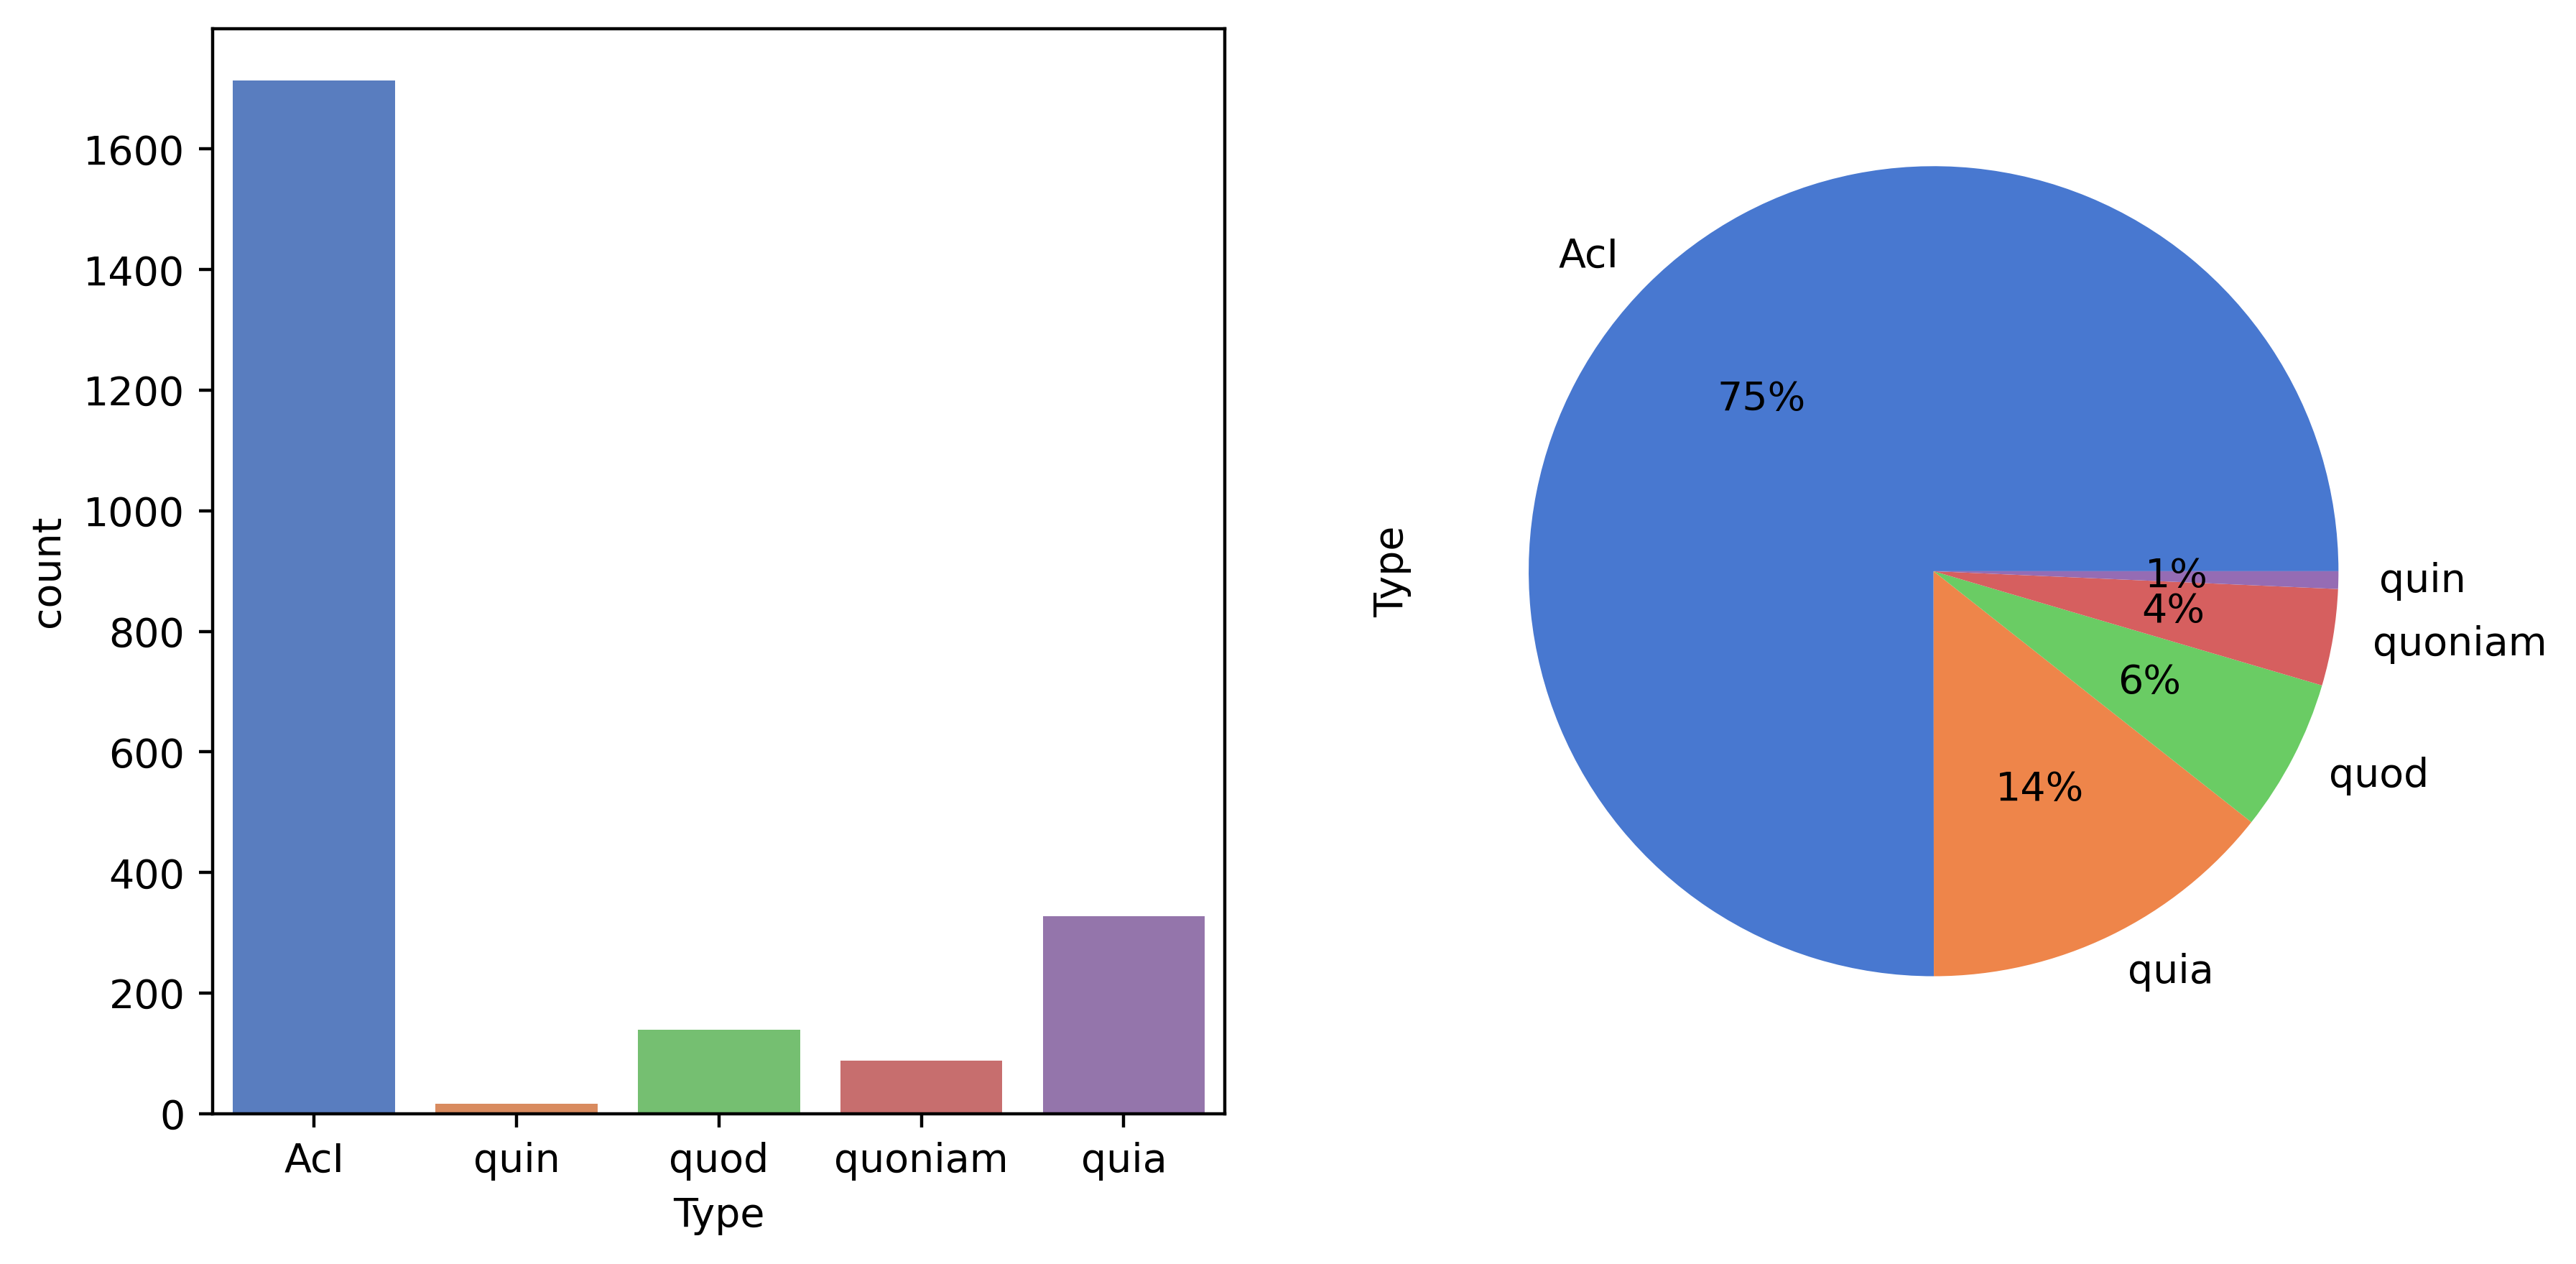
\includegraphics[width=\textwidth,height=\textheight,keepaspectratio]{graphs/type.png}
\end{center}
\end{frame}

\begin{frame}
\frametitle{Type by era}
\begin{center}
    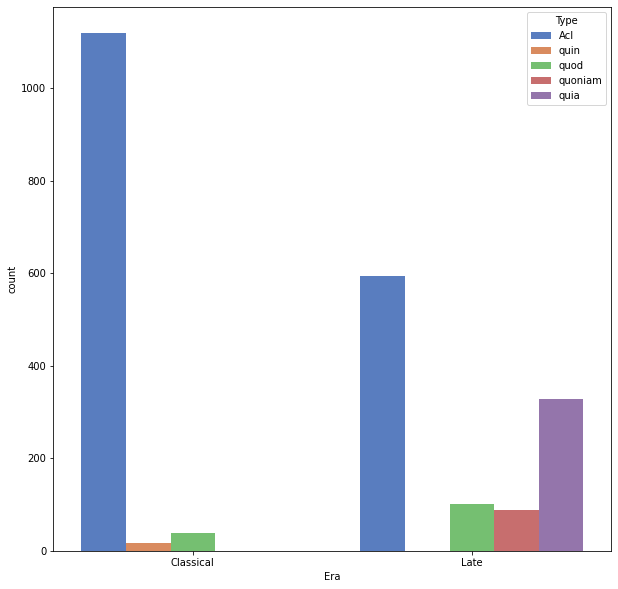
\includegraphics[width=\textwidth,height=0.8\textheight,keepaspectratio]{graphs/type_by_era.png}
\end{center}
\end{frame}

\begin{frame}
\frametitle{Type by author}
\begin{center}
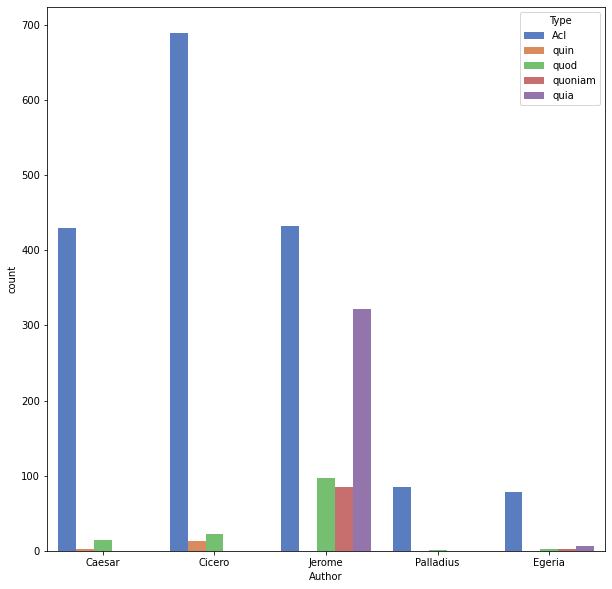
\includegraphics[width=\textwidth,height=0.8\textheight,keepaspectratio]{graphs/type_by_auth.png}
\end{center}
\end{frame}

\begin{frame}
\frametitle{The problem with Jerome}
Jerome was known for preserving the original syntax

Greek has complementizers like \textit{h\'oti} and \textit{g\'ar}

Therefore, his high use of complementizers may not reflect a wholly-Latin development

Would need to do more research into Greek
\end{frame}

\begin{frame}
\frametitle{Voice by type}
\begin{center}
    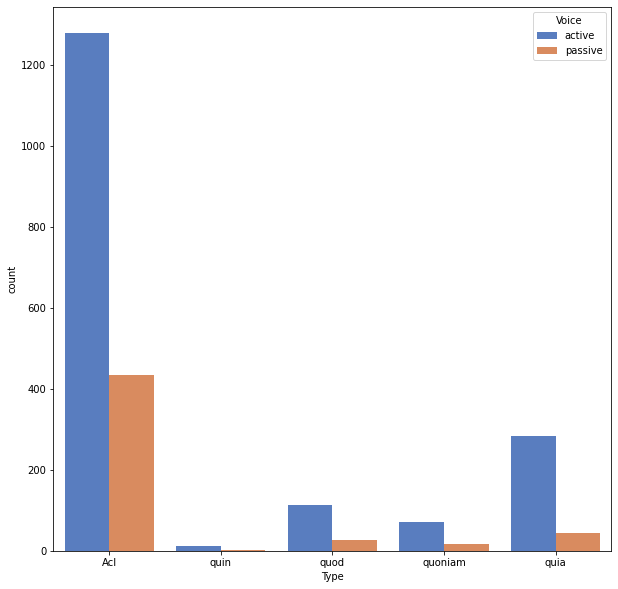
\includegraphics[width=\textwidth,height=0.8\textheight,keepaspectratio]{graphs/voice_by_type.png}
\end{center}
\end{frame}

\begin{frame}
\frametitle{Tense by type}
\begin{center}
    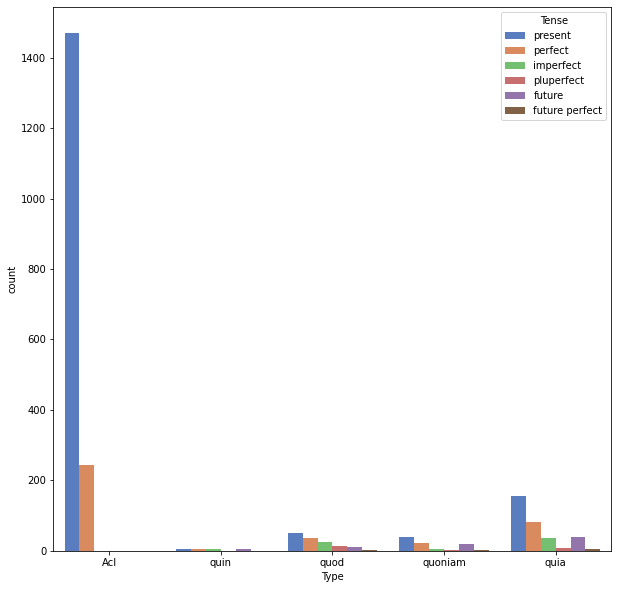
\includegraphics[width=\textwidth,height=0.8\textheight,keepaspectratio]{graphs/tense_by_type.png}
\end{center}
\end{frame}

\begin{frame}
\frametitle{Mood by type and author}
\begin{center}
    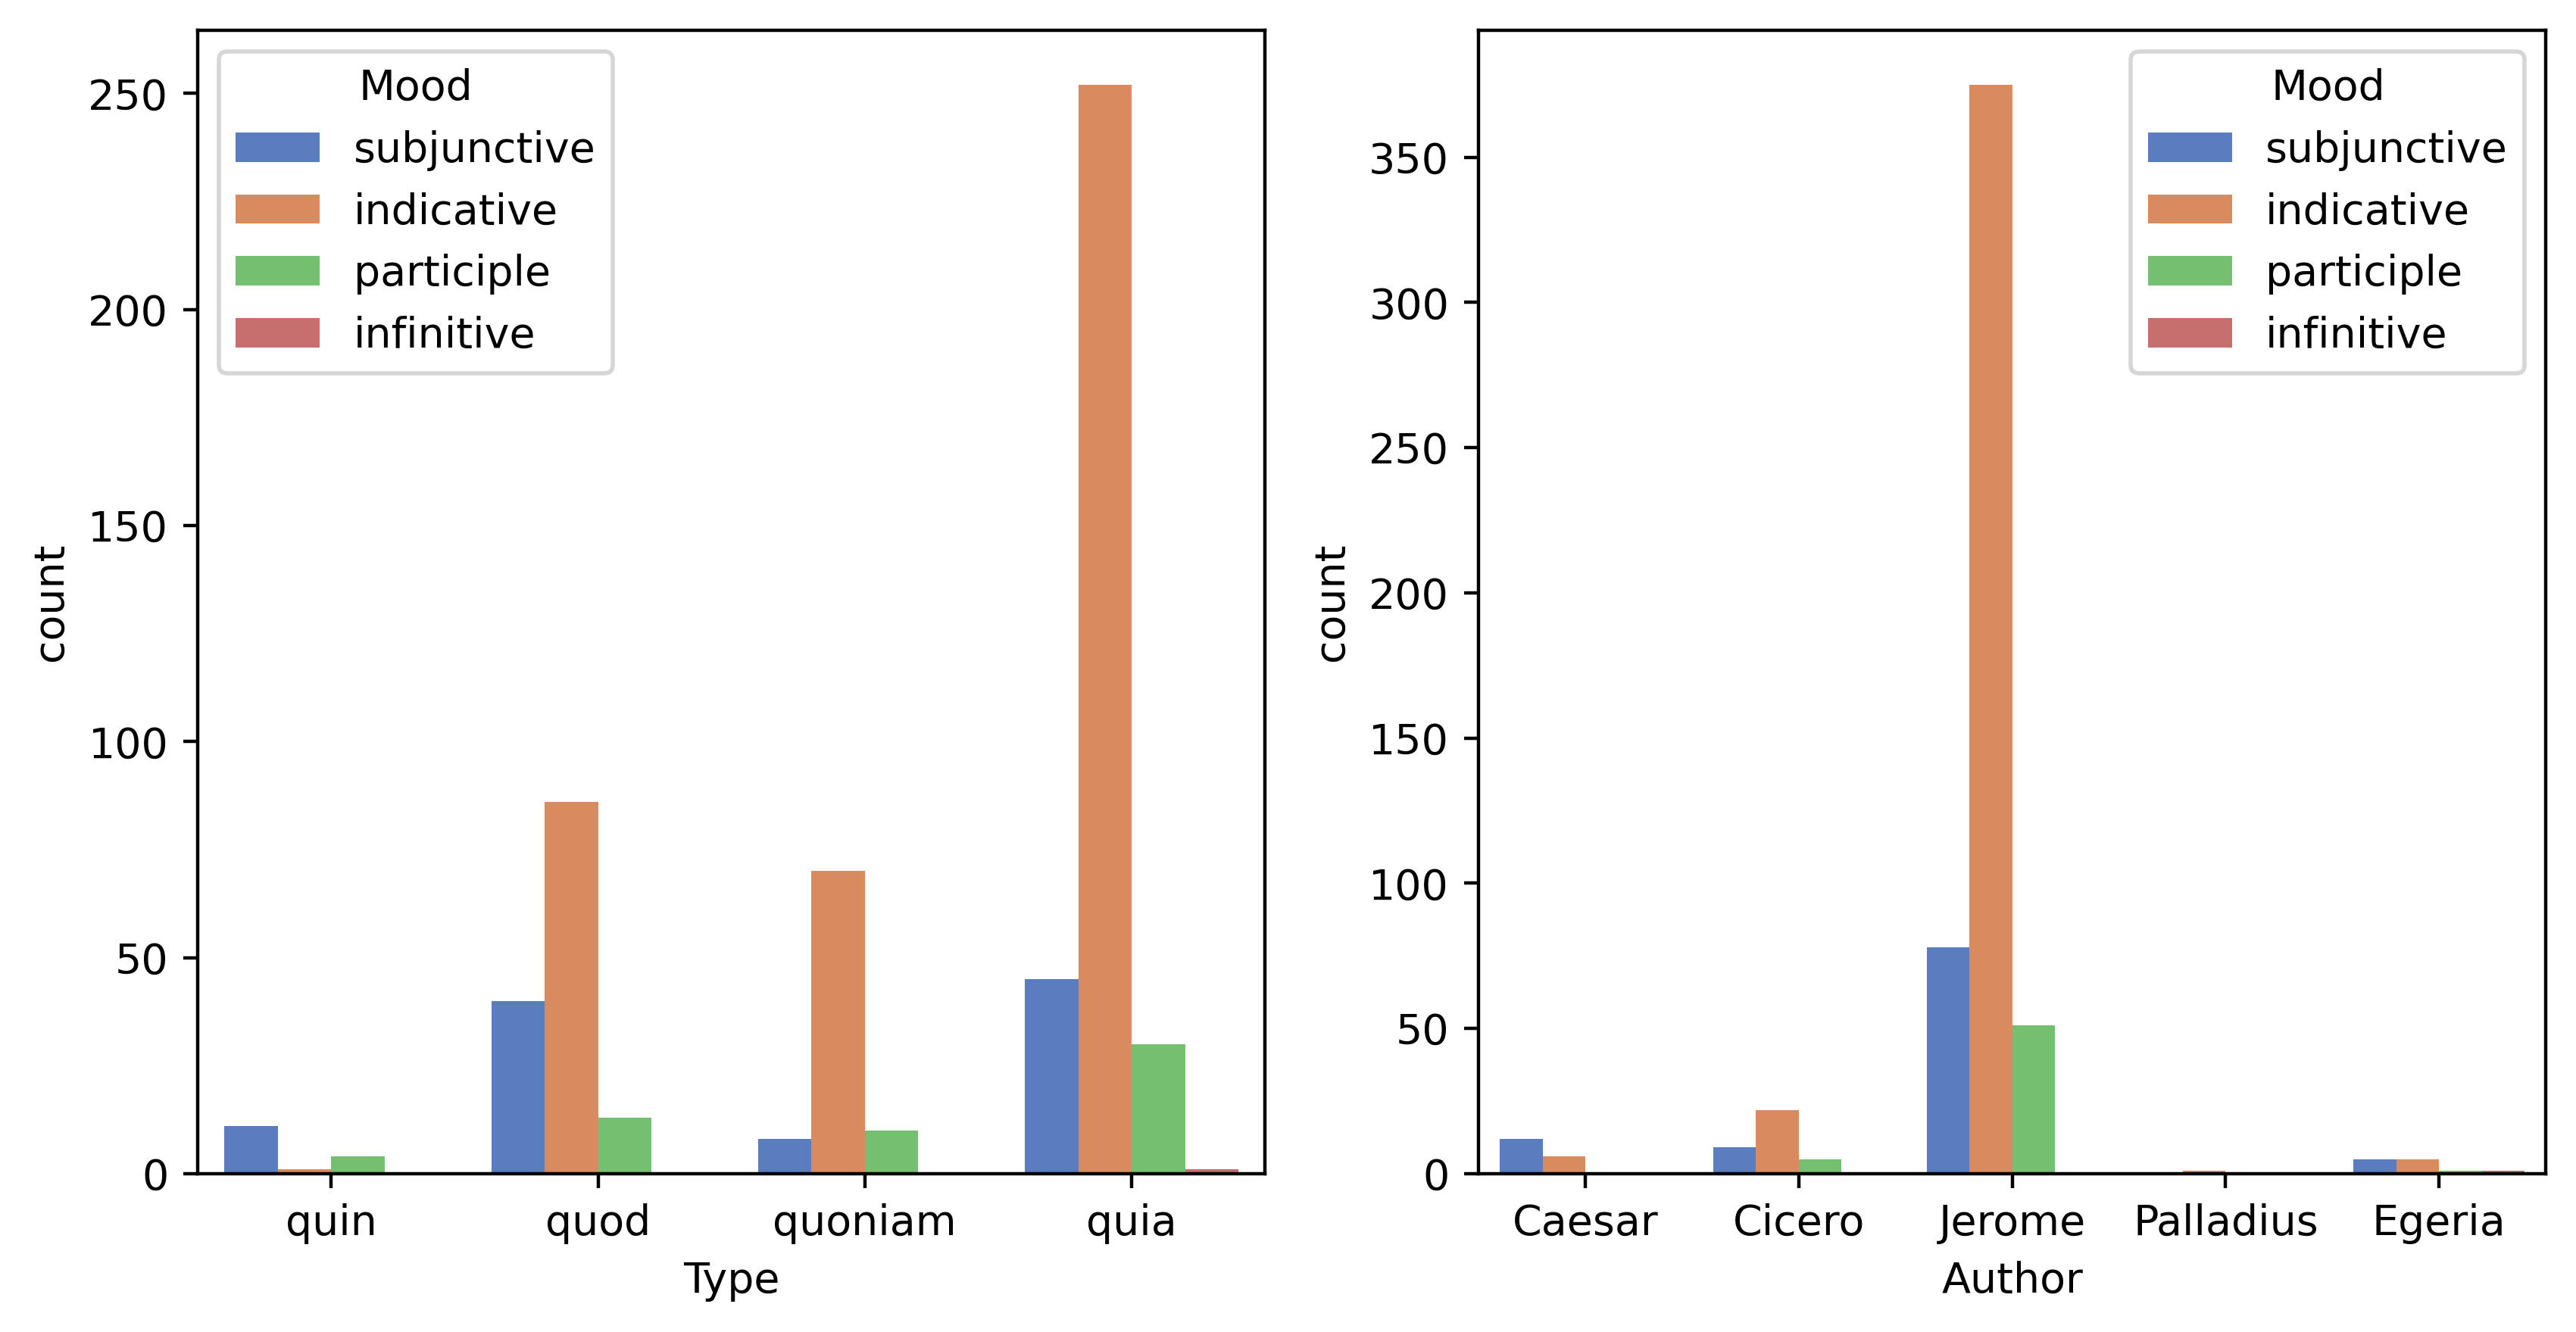
\includegraphics[width=\textwidth,height=\textheight,keepaspectratio]{graphs/mood_by_type_auth.png}
\end{center}
\end{frame}

\begin{frame}
\frametitle{Tense and voice by era}
In modern Romance languages, the future tense and passive do not survive

(In most Romance languages, the future tense derives from fusion of the infinitive with the verb \textit{habeō} `I have')

Are these forms less frequent in later works?
\end{frame}

\begin{frame}
\frametitle{Tense and voice by era}
\begin{center}
    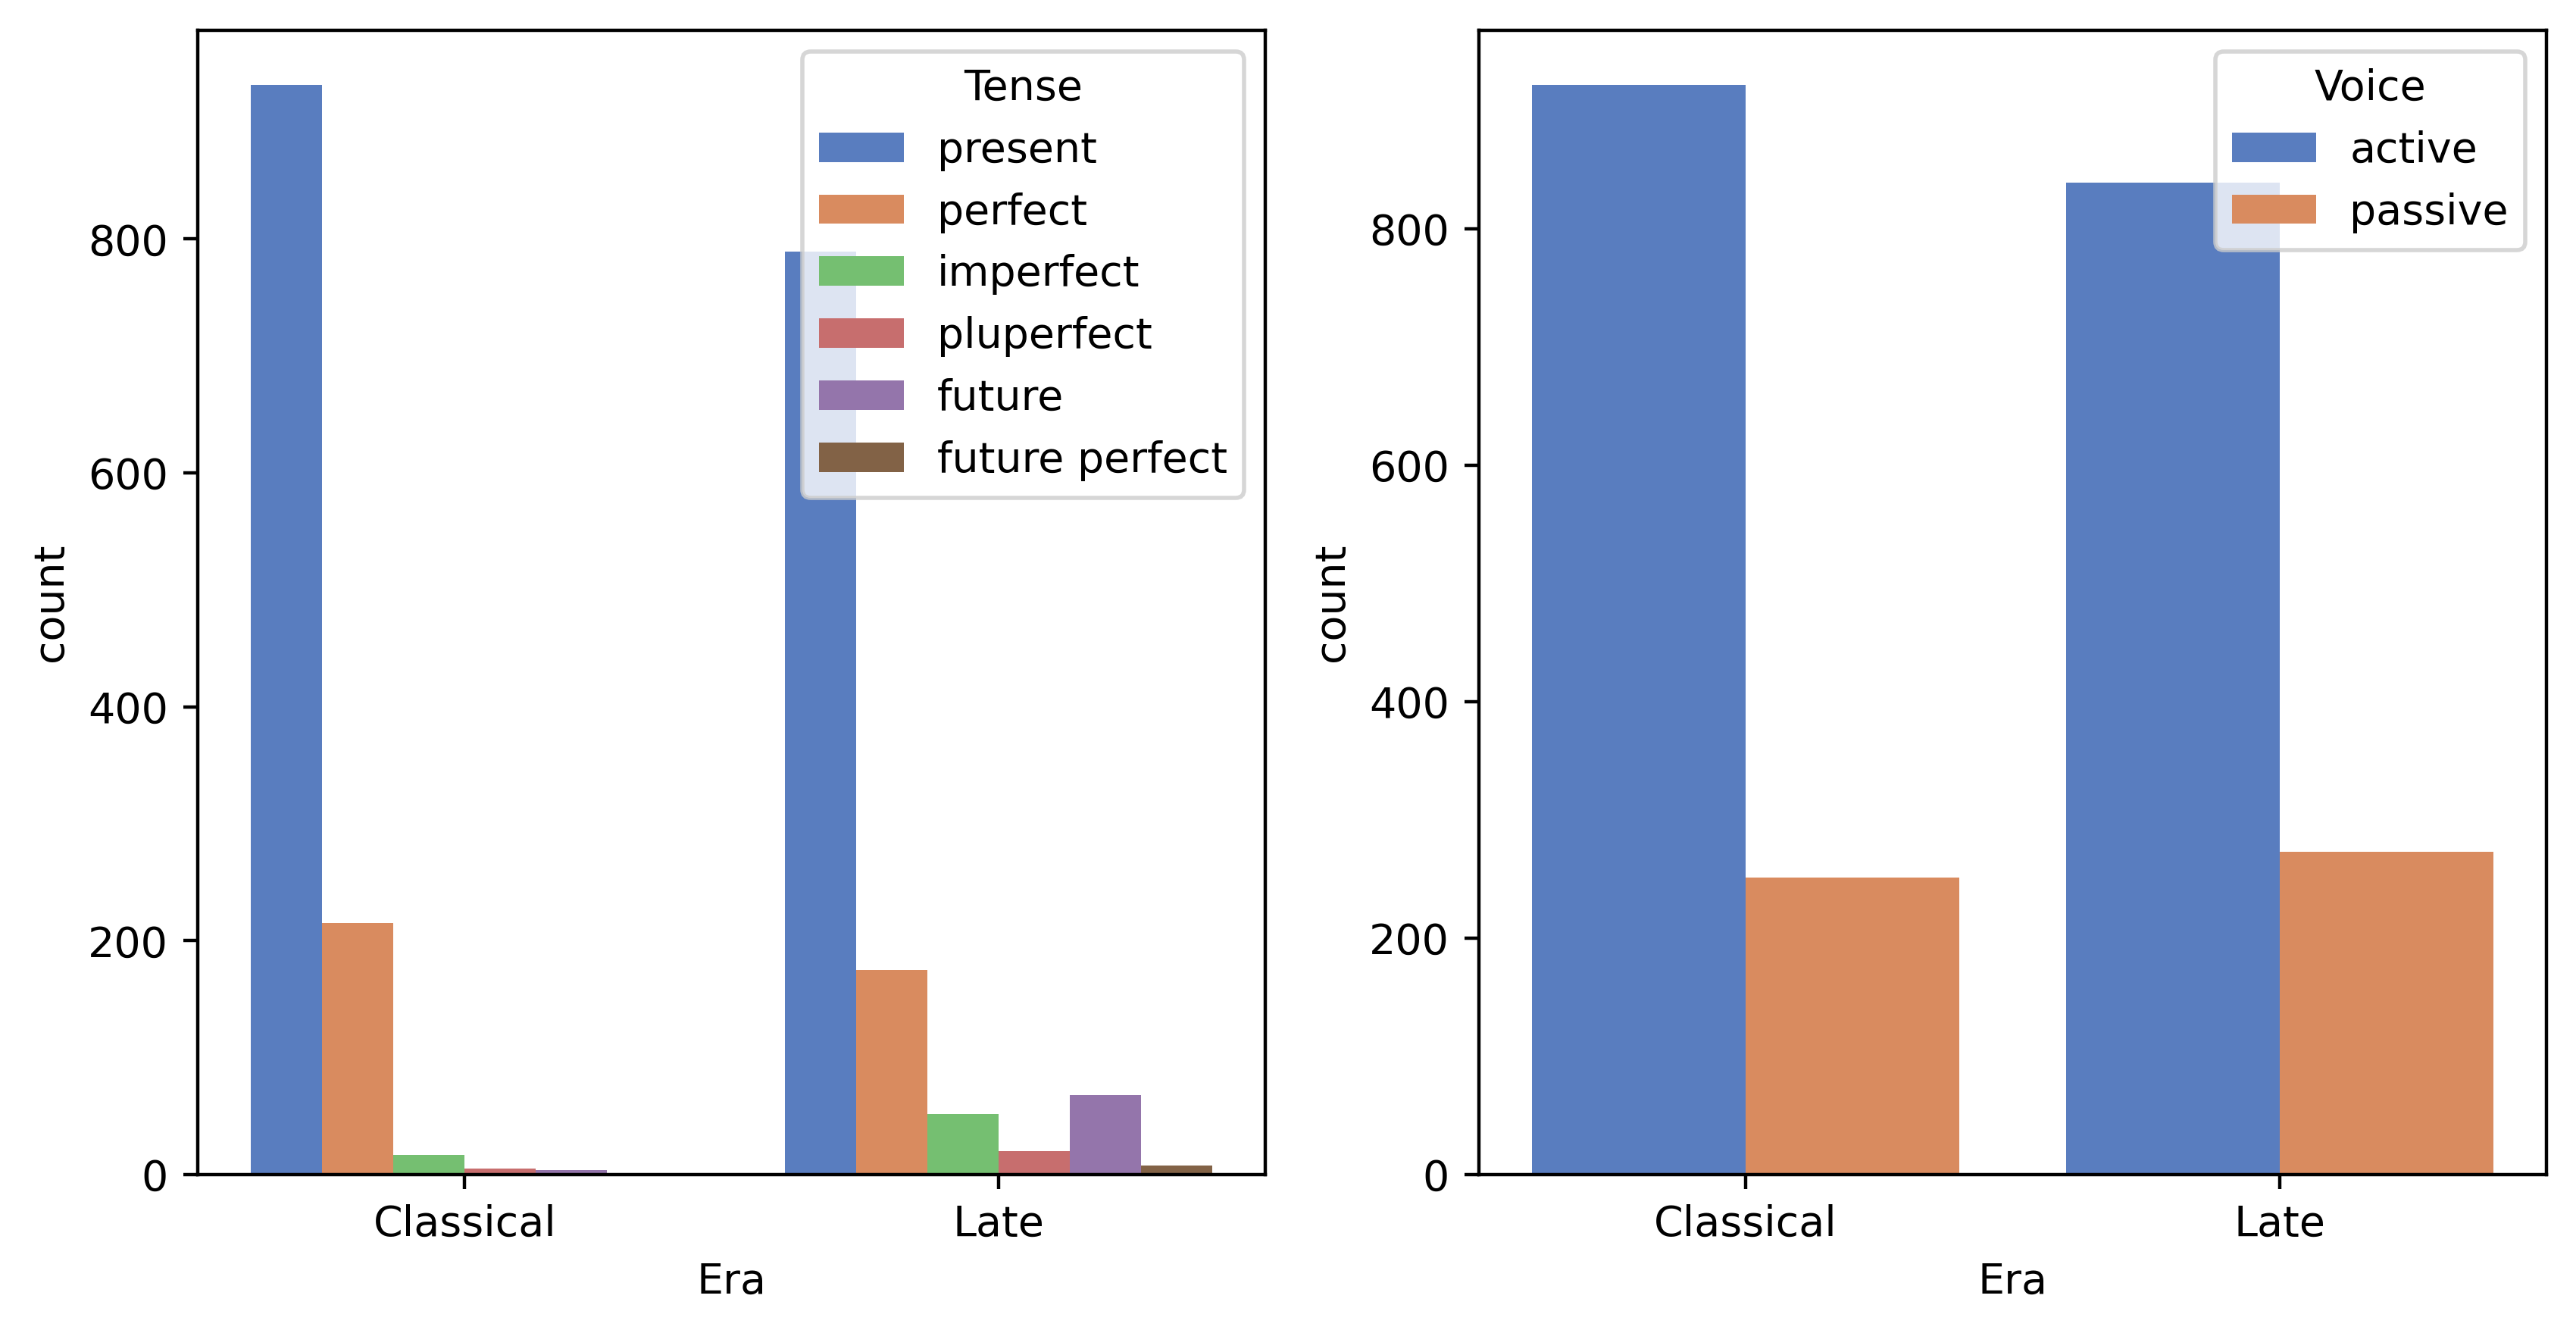
\includegraphics[width=\textwidth,height=\textheight,keepaspectratio]{graphs/tense_voice_by_era.png}
\end{center}
\end{frame}

\begin{frame}
\frametitle{Tense and voice by era}
Perhaps even the `late' texts predate this development

Possibly the effect of a written register
\end{frame}

\begin{frame}
\frametitle{Facienda -- what must be done}
Look more into the `problem with Jerome'

Finish up analysis

Look into introductory verbs -- if there is time

\end{frame}

\end{document}
